% fig02_density_sweep.tex — the marginal (confounded) rise of integration with
% density. Standalone; `make figures` -> figures/fig02_density_sweep.pdf.
% Data (exact enumeration; p=0.4 point = mean of the two equal-n F3 halves):
%   B category Phi : (0.2, 0.3875) (0.4, 0.8667) (0.6, 1.0)
%   C topology Phi : (0.2, 0.2333) (0.4, 0.7417) (0.6, 0.9583)
\documentclass[tikz,border=4pt]{standalone}
\usepackage{pgfplots}
\pgfplotsset{compat=1.18}
\begin{document}
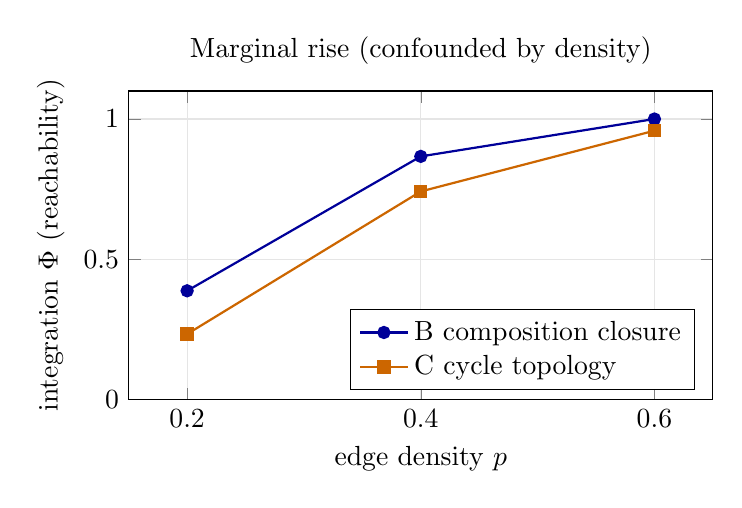
\begin{tikzpicture}
  \begin{axis}[
    width=9cm, height=5.5cm,
    xlabel={edge density $p$}, ylabel={integration $\Phi$ (reachability)},
    xmin=0.15, xmax=0.65,
    ymin=0, ymax=1.1,
    xtick={0.2,0.4,0.6},
    grid=both, grid style={gray!20},
    legend pos=south east, legend cell align=left,
    title={Marginal rise (confounded by density)},
  ]
    \addplot[mark=*, thick, color=blue!60!black] coordinates {
      (0.2, 0.3875) (0.4, 0.8667) (0.6, 1.0)
    };
    \addlegendentry{B composition closure}
    \addplot[mark=square*, thick, color=orange!80!black] coordinates {
      (0.2, 0.2333) (0.4, 0.7417) (0.6, 0.9583)
    };
    \addlegendentry{C cycle topology}
  \end{axis}
\end{tikzpicture}
\end{document}
